\documentclass[tikz,border=3mm]{standalone}
\usepackage{pgfplots}

\pgfplotsset{compat=1.16}
\pgfplotsset{
    colormap={genqs}{
        rgb255=(0,0,128)
        rgb255=(0,0,128)
        rgb255=(0,0,128)
        rgb255=(128,0,0)
        rgb255=(0,128,32)
        rgb255=(0,128,32)
        rgb255=(0,128,32)
        rgb255=(0,128,32)
        rgb255=(0,128,32)
        rgb255=(0,128,32)
        rgb255=(0,128,32)
        rgb255=(0,128,32)
        rgb255=(0,128,32)
        rgb255=(0,128,32)
        rgb255=(0,128,32)
        rgb255=(0,128,32)
        rgb255=(0,128,32)
        rgb255=(0,128,32)
        rgb255=(128,0,0)
        rgb255=(0,0,128)
        rgb255=(0,0,128)
        rgb255=(0,0,128)
    },
}
    
\begin{document}
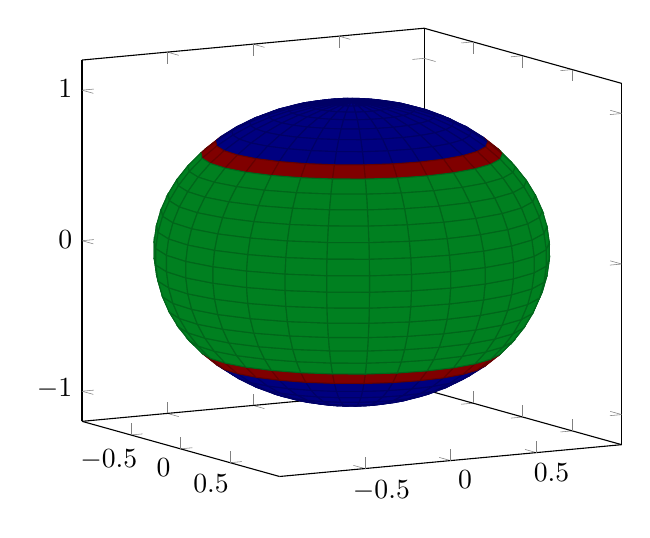
\begin{tikzpicture}
\begin{axis}[view={60}{10},colormap access=piecewise const]
    \addplot3 [
        surf,
        z buffer=sort,
        samples=30,
        domain=0:2*pi,
        y domain=0:pi
    ] (
        {cos(deg(x)) * sin(deg(y))},
        {sin(deg(x)) *sin(deg(y))},
        {cos(deg(y))}
    );
\end{axis}
\end{tikzpicture}

\end{document}